\documentclass{article}
\usepackage[utf8]{inputenc}
\usepackage{amsmath}
\usepackage{graphicx}
\usepackage[margin=1.2in]{geometry}
\usepackage{siunitx}
\usepackage{amsmath,amsthm,amsfonts,amssymb,mathrsfs}
\usepackage{physics}
\usepackage{enumitem}
\usepackage{hyperref}
\usepackage{float}


\title{Deep learning approach to crystal stability}
\author{Love Pettersson }
\date{February 2020}

\begin{document}

\maketitle
\newpage
\section{Abbreviations}
ANN: Artificial neural network \\
DFT: Density functional theory \\
MAE: Mean absolute error \\
MSE: Mean squared error \\
MLP: Multi-layer perceptron \\
CNN: Convolutional neural network

\newpage
\section{Introduction}


\section{Artificial neural networks}
Artificial neural networks are computational architectures, modelled after inspiration drawn from the human brain and how it performs different tasks \cite{McCulloch1943}. In analogy to the biological neurons ANNs are composed of a large amount of "artificial neurons", which, like the biological neurons, are the working units of the network. The strength of the interconnection between the artificial neurons is regulated by the "synaptic weights". These are modified through a learning process, such that the network as a whole performs well on the desired task. Specifically these two attributes of neural networks, (1) its abilities to learn and (2) its massive architectures of interconnected artificial neurons, that shows resemblance to the human brain \cite{Simonhaykin}.\\


 
\subsection{The Perceptron}
The explanation above is to some degree abstract. To make it more concrete, we will introduce and explain the perceptron. Since it is the most basic ANN architecture, composed of only one artificial neuron, it serves as a great example to clarify the inner mechanisms of ANNs. In figure 1, an illustration of the perceptron is shown. 
\begin{figure}[h!] 
	\centering
	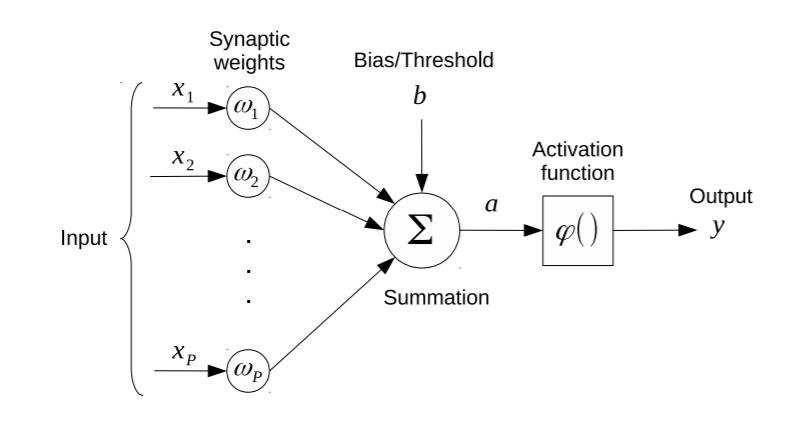
\includegraphics[width=0.8\textwidth]{Simple_preceptron.png}
	\caption{Picture illustrating the simple perceptron \cite{Lecturenotes}.}
	\label{fig:Simple-perceptron}
\end{figure} \\
The perceptron performs the following operations:
\begin{equation}
    a=\sum_{n=1}^{P}x_nw_n+b 
\end{equation}
\begin{equation}
     y=\varphi(a)
\end{equation}
Starting with an input vector $\Vec{x}$, the perceptron performs a weighted sum with weight vector $\Vec{w}$ plus a bias term b. The sum is passed through the function $\varphi$ such that an output y is produced. The weight vector $\Vec{w}$ is what is referred to as the "synaptic weight" and the function $\varphi$ is usually denoted the name "activation function". There are various of popular activation functions, which are chosen depending on the task. For example, the output activation function for a regression problem, the linear activation function $\varphi(a)=a$ is a convenient choice since it can take any numerical value. However, for a binary classification problem, the sigmoid function $\varphi(a)=\frac{1}{1+e^{-a}}$ is more applicable since it is bounded between zero and one. Usually, the two different classes in binary classification are represented by zero or one, respectively \cite{Lecturenotes}. \\ %maybe no need to explain?
The perceptron, although being a great first example for understanding the operations executed inside ANNs, is not enough to perform relevant tasks. Instead, larger and more complex architectures must be used. The architectures covered in this work are the multi-layer perceptron (MLP) and the convolutional neural network (CNN). %maybe skip last sentence?


%explain what it does

\subsection{Multi-layer perceptron}
The multi-layer perceptron architecture is a generalisation of the simple perceptron \cite{Simonhaykin}. It is, instead of being composed of only one artificial neuron, comprised of many of these. Rather than just consisting of one output layer, it is constructed with hidden layers. The amount of hidden layers determines the depth of the network, from this phrasing the name "Deep learning" originates \cite{Deeplearningbook}. Figure 2 shows an illustration of an MLP with two hidden layers.
\begin{figure}[h!] 
	\centering
	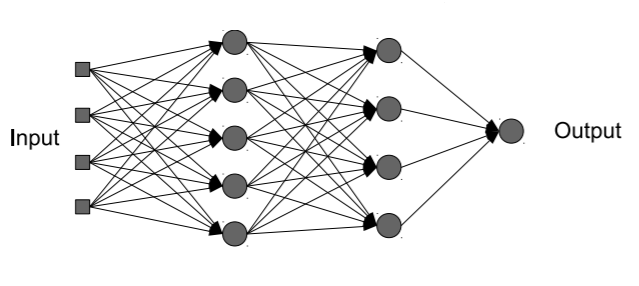
\includegraphics[width=0.8\textwidth]{Multi_layer_perceptron.png}
	\caption{Illustration of a multi-layer perceptron with two hidden layers. \cite{Lecturenotes}}
	\label{fig:Multilayer-perceptron}
\end{figure}\\

The intent of introducing the hidden layers is to, within each layer, gradually extract important features of the input. By extracting features in the hidden layers, the MLP is able to solve complex problems. Moreover, we require the activation functions in the hidden layers to be non-linear. The output of a network using linear activation functions in the hidden layer would be represented by a linear combination of these. Since this output would be simply linear, it can can be represented by a network with only one output layer. For large networks, which are of interest in this work, the rectifier activation function (ReLU) $\varphi(a)=$max(0,a) is very popular. It has many advantageous features, which will be apparent in the discussion of training the network and achieving a good generalisation. %maybe skip this part


\subsection{Convolutional neural networks}
Convolutional neural networks (CNN) are a specialised type of network. It is originally designed for image analysis, but is frequently used in many different applications where the input has a grid-like topology \cite{Deeplearningbook}. Instead of performing a matrix multiplication with the input, as seen in equation 1 for the simple perceptron, the CNN performs the mathematical operation named convolution.
\begin{equation}
    a=(x\ast w)(k)=\sum_{n}x(n)w(k-n)
\end{equation}
The function x is the input and the function w, when working with CNNs, is referred to as the kernel. Furthermore, this operation can be generalised to higher dimensions, hence CNNs provide a tool to work with inputs of dimensions higher than one.\\
Although the above explanation is correct, one can also describe the operation performed by CNNs in the terminology of MLPs. The ordinary MLP is said to be fully connected, meaning that every hidden node is connected to the full input vector. The CNN can be seen as an MLP which is sparsely connected and has hidden nodes that share weights. 
\\
After the convolution stage, the output is passed through an activation function. As for large MLPs, the ReLU function is frequently used. Further, it is possible to include a third stage known as pooling. The pooling operation assigns the hidden nodes a different value depending on their neighbours. For instance, max pooling assigns the hidden nodes the maximum value of their neighbours. This is of interested when only a specific feature needs to be extracted and not its placement.










%Introduce the name node?

\subsection{Training network}

\subsection{Overfitting and generalisation}















\bibliographystyle{apalike}
\bibliography{references}
\end{document}
